\documentclass[12pt, twocolumn]{article}   	
\usepackage{amssymb}
\usepackage[hmarginratio=1:1,top=32mm,columnsep=20pt]{geometry}
\usepackage{graphicx}
\usepackage{multicol} % Used for the two-column layout of the document
\usepackage{hyperref} %Used to support hyperlinks in the document
\hypersetup{colorlinks=true, urlcolor=blue}
% -----------------------------------------------------------------------------------------------
% DOCUMENT
% -----------------------------------------------------------------------------------------------					
\begin{document}
% ----------------------------------------------------------------------------------------------
% TITLE SECTION
% ---------------------------------------------------------------------------------------------- 
\twocolumn[{%
 \centering
 \LARGE \textbf{Cloud of Things - Preliminary Report }\\[1em]
 \large \textsc{Marcus Gomes}\\[2em]
 }]
% -----------------------------------------------------------------------------------------------
% ABSTRACT
% -----------------------------------------------------------------------------------------------
\begin{abstract}
\textbf{\textit{Cloud of Things is an automated infrastructure platform that combines the technologies of Cloud Computing and the Internet of Things to capture information about relevant physical objects in a given space.
Before to start the platform development, our first assignment in the master thesis is a challenge in that, during a month, we have to develop a prototype that shows our vision about the work to be realized. Thus, this report presents the work realized during this month, the obtained results and some directions regarding the future work to be realized.}}
\end{abstract}
% -----------------------------------------------------------------------------------------------
% INTRODUCTION
% ------------------------------------------------------------------------------------------------
\section{Introduction}
To start the work in the master thesis dissertation, in the beginning of the semester we were challenged to develop a prototype that demonstrates our ideas about the purpose of our theme.
Thus, during the past month, my work was focused in develop a prototype of  Cloud of Things, an automated infrastructure platform that combines two emerging technologies, the Cloud Computing, that
allows to make provisioning of virtual machines and software configuration in a fast way, and the Internet of Things, that takes advantage from identification technologies, such as RFID, to capture information about
relevant physical objects in a given space.
% ------------------------------------------------------------------------------------------------
%  MOTIVATION
% ------------------------------------------------------------------------------------------------
 \section{Motivation}
 The main motivation for this challenge was try to understand with more detail the work to be realized, its limitations and what can be done to cover some of this limitations.\\
 The starting point of the work was research the existent components that could be used in the development, namely the Cloud providers and frameworks to capture information about physical objects in a certain environment.
 Regarding the Cloud providers, the research was in a certain way very easy, mainly because the amount of information that is available on the Web and because the previous knowledge that i have about the subject. As result, 
 the most relevant providers regarding referencies, documentation and quality of service was Google Compute Engine, Amazon Web Services and Microsoft Azure. Regarding the frameworks to make the capture the information about
 physical objects, in a previous agreement made with the advisors the choice was to use Fosstrak, an open source RFID software platform.\\
 The second step was figure out how to automate the deploy and configuration of Cloud of Things. The approach was make use of a tool that automates the infrastructure configuration and management, like Ansible, Salt, Puppet and Chef. 
 In the \textbf{Development} section, the tool to achieve that will be described with further detail.
 % ------------------------------------------------------------------------------------------------
 % DEVELOPMENT
 % ------------------------------------------------------------------------------------------------   
 \section{Development}
 Before to start the prototype development, it was necessary to choose the tools to do so. To choose the IT automation platform and the Cloud provider, aspects like the integration between the platforms and the learning curve were considered.
 Initially the automation tools considered to use in the development were Puppet and Chef. After analyze the \textit{pros} and \textit{cons} of each platform, Puppet was chosen due the amount of documentation available, the maturity of the platform 
 and because Puppet is more friendly to be used by beginners. Regarding the Cloud provider the choice relies on Google Compute Engine (GCE), mainly because Puppet comes prepared to be integrated with Google Compute Engine.\\
 Next a more detailed explanation of the development process will be given. 
 \subsection{Puppet \& GCE}
 To automate the provisioning and configuration of the instances at the Cloud, it was needed integrate Puppet with Google Compute Engine. But first, it was needed to understand how Puppet works.\\
 After reading the documentation available in \href{https://docs.puppetlabs.com/}{Puppet Labs}, comprehend how Puppet works becomes more trivial, but experimentation is essential to really understand how the framework operates.\\
 
 \begin{figure}[htb!] %  figure placement: here, top, bottom, or page
    \centering
    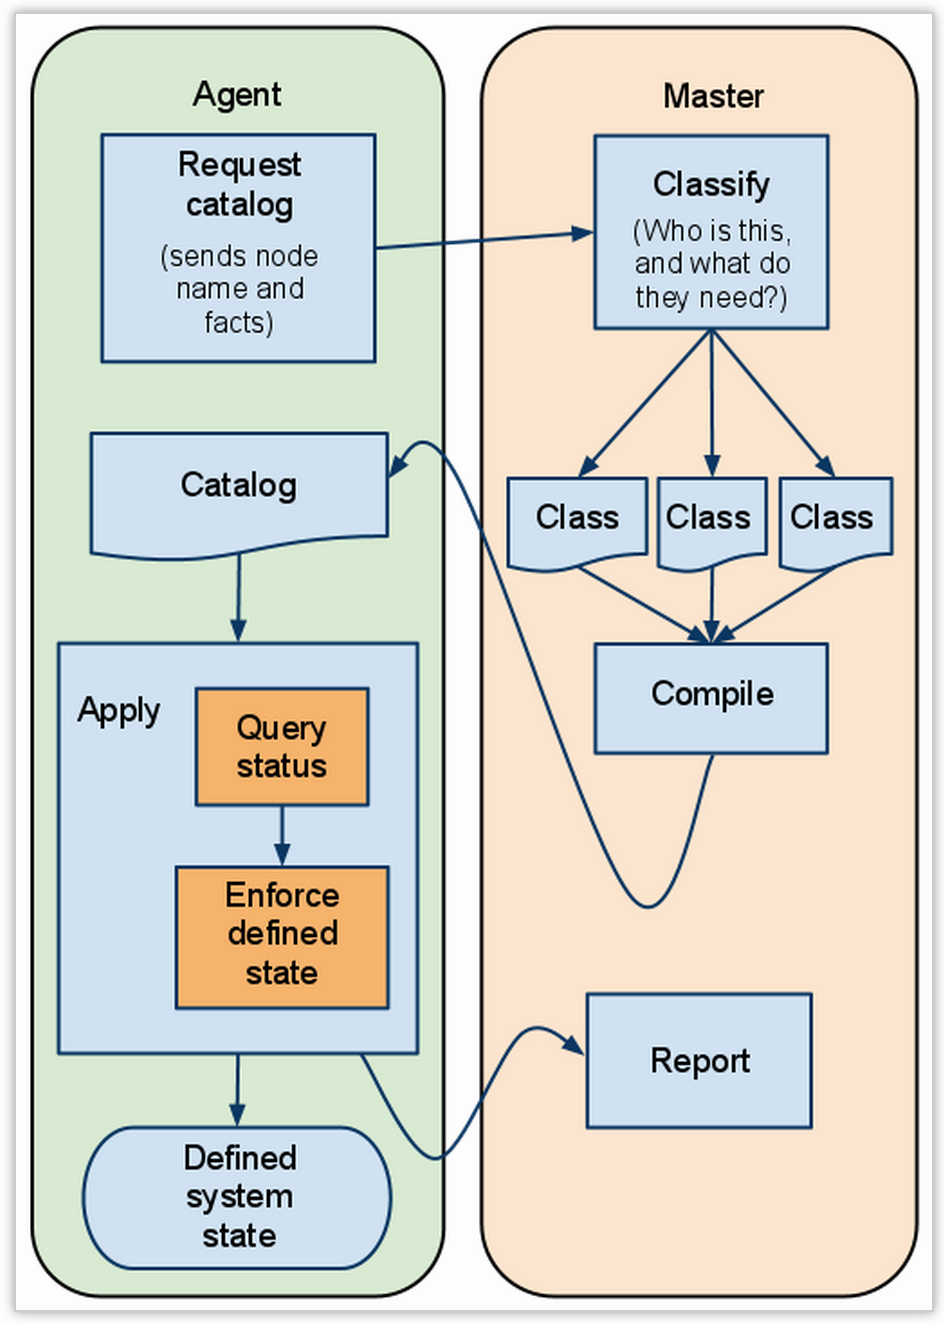
\includegraphics[width=.45\textwidth]{puppet} 
    \caption{Puppet Master/Agent Interaction}
    \label{fig:puppet}
 \end{figure} 
 
Puppet has two main components, the Puppet Master and the Puppet Agent. The Puppet Master is a server responsible to store the configuration scripts, the Manifests, that will be pulled by the Puppet Agents, through the Puppet Master is also possible verify the actual system state. The Puppet Agent is a server that is configured by pulling the the configuration files from the Puppet Master, and between regular intervals the Puppet Agent must sent a report about its status to the Puppet Master. A more detailed 
 explanation about the interaction between the Puppet Master and the Puppet Agent is demonstrated in the picture above.\\
 Thus, the desired automation is achieved by Puppet via Puppet Manifests, that is the way to tell to Puppet what i want installed in a machine. The manifest  contains a description of the components to be installed and the dependencies between these
 components. Fortunately due the integration between Puppet and GCE, Puppet Labs already provides via  \href{https://forge.puppetlabs.com/}{Puppet Forge} a module to configure the instances to be provisioned.\\
 Therefore, to configure the instances the procedure was use the \href{https://forge.puppetlabs.com/puppetlabs/gce_compute}{GCE Module} and the documentation provided by Puppet Forge to configure and deploy the instance on the Google Cloud Platform.          
 \subsection{Fosstrak}
 To configure and deploy the Fosstrak platform at the provisioned instances was more complicated, because Puppet does't provides any module to configure the platform at the instances. The solution was write the Puppet Manifests to install and configure all the components required to deploy Fosstrak, namely the Apache Tomcat web server , the MySQL Database and the Fosstrak EPCIS repository. The configuration scripts was based on the documentation provided by the \href{https://code.google.com/p/fosstrak/wiki/EpcisDeveloperGuide}{Fosstrak EPCIS Developer Guide}.
 \subsection{Testing}
 After the integration between the platforms was finished, it was time to test the system and confirm if the integration was successfully implemented or not. For that, Fosstrak already provides the a Capture Client to send events to the repository and a Query 
 client to browse a repository. After follow the instructions in the Fosstrak User Guide, the tests to capture and browse the repository creates at the Google Clod runs successfully.\\
 The picture that follows shows the Fosstrak Architecture, and its possible to see how the Fosstrak Capture Client and Query Client interact with the Fosstrak repository.
 
 \begin{figure}[htb!] %  figure placement: here, top, bottom, or page
    \centering
    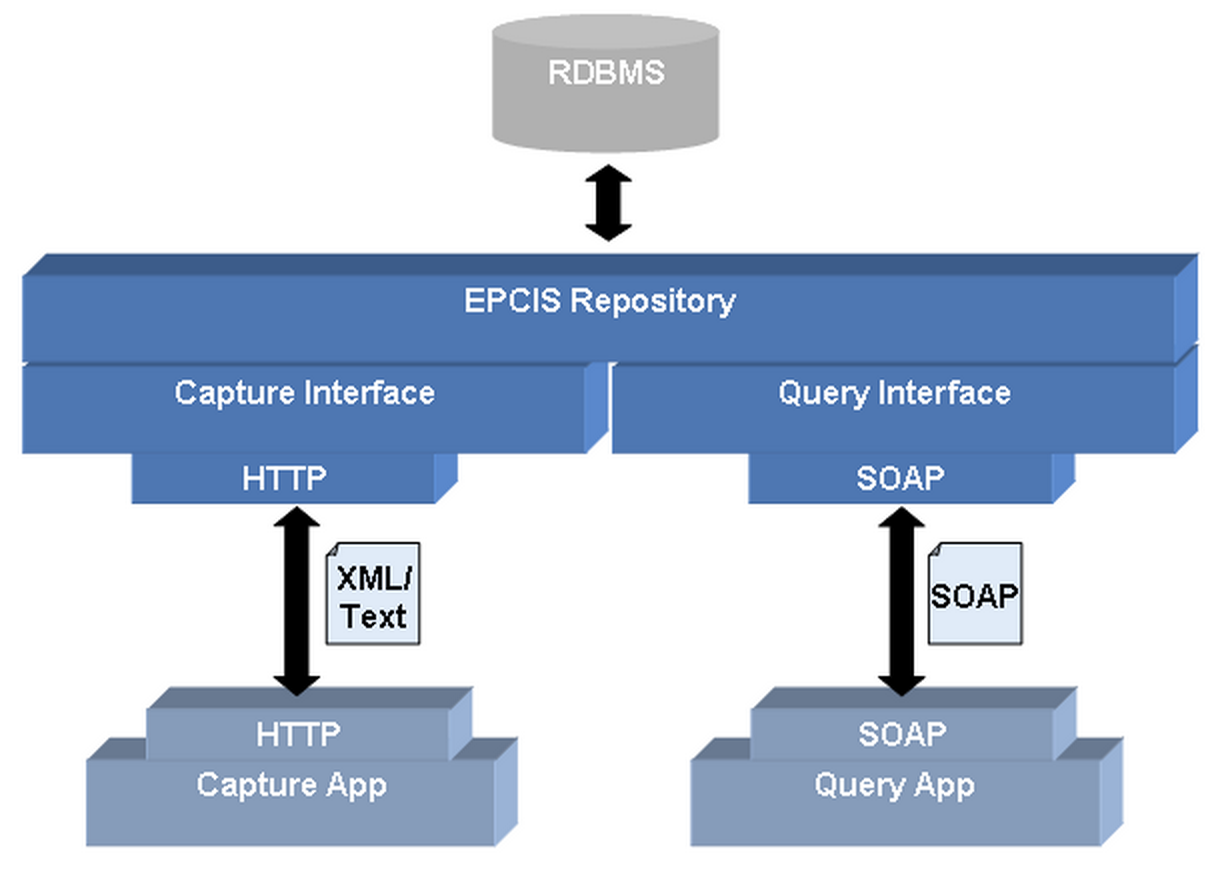
\includegraphics[width=.45\textwidth]{fosstrak} 
    \caption{Fosstrak Architecture}
    \label{fig:fosstrak}
 \end{figure} 	 
 
 All the developed work could be found in the \href{https://github.com/mvpgomes/cloud-of-things}{Cloud of Things} GitHub repository. 
 % ----------------------------------------------------------------------------------------------
 % DEMONSTRATION
 % ----------------------------------------------------------------------------------------------
 \section{Demonstration}
 The challenge ends with a demonstration for the advisors and the colleagues. In this demonstration the objective was to show the developed work, more precisely, show a scenario were a technician configure and deploy the platform in a Smart Space, as showed on the image below.
 
 \begin{figure}[htb!]
    \centering
    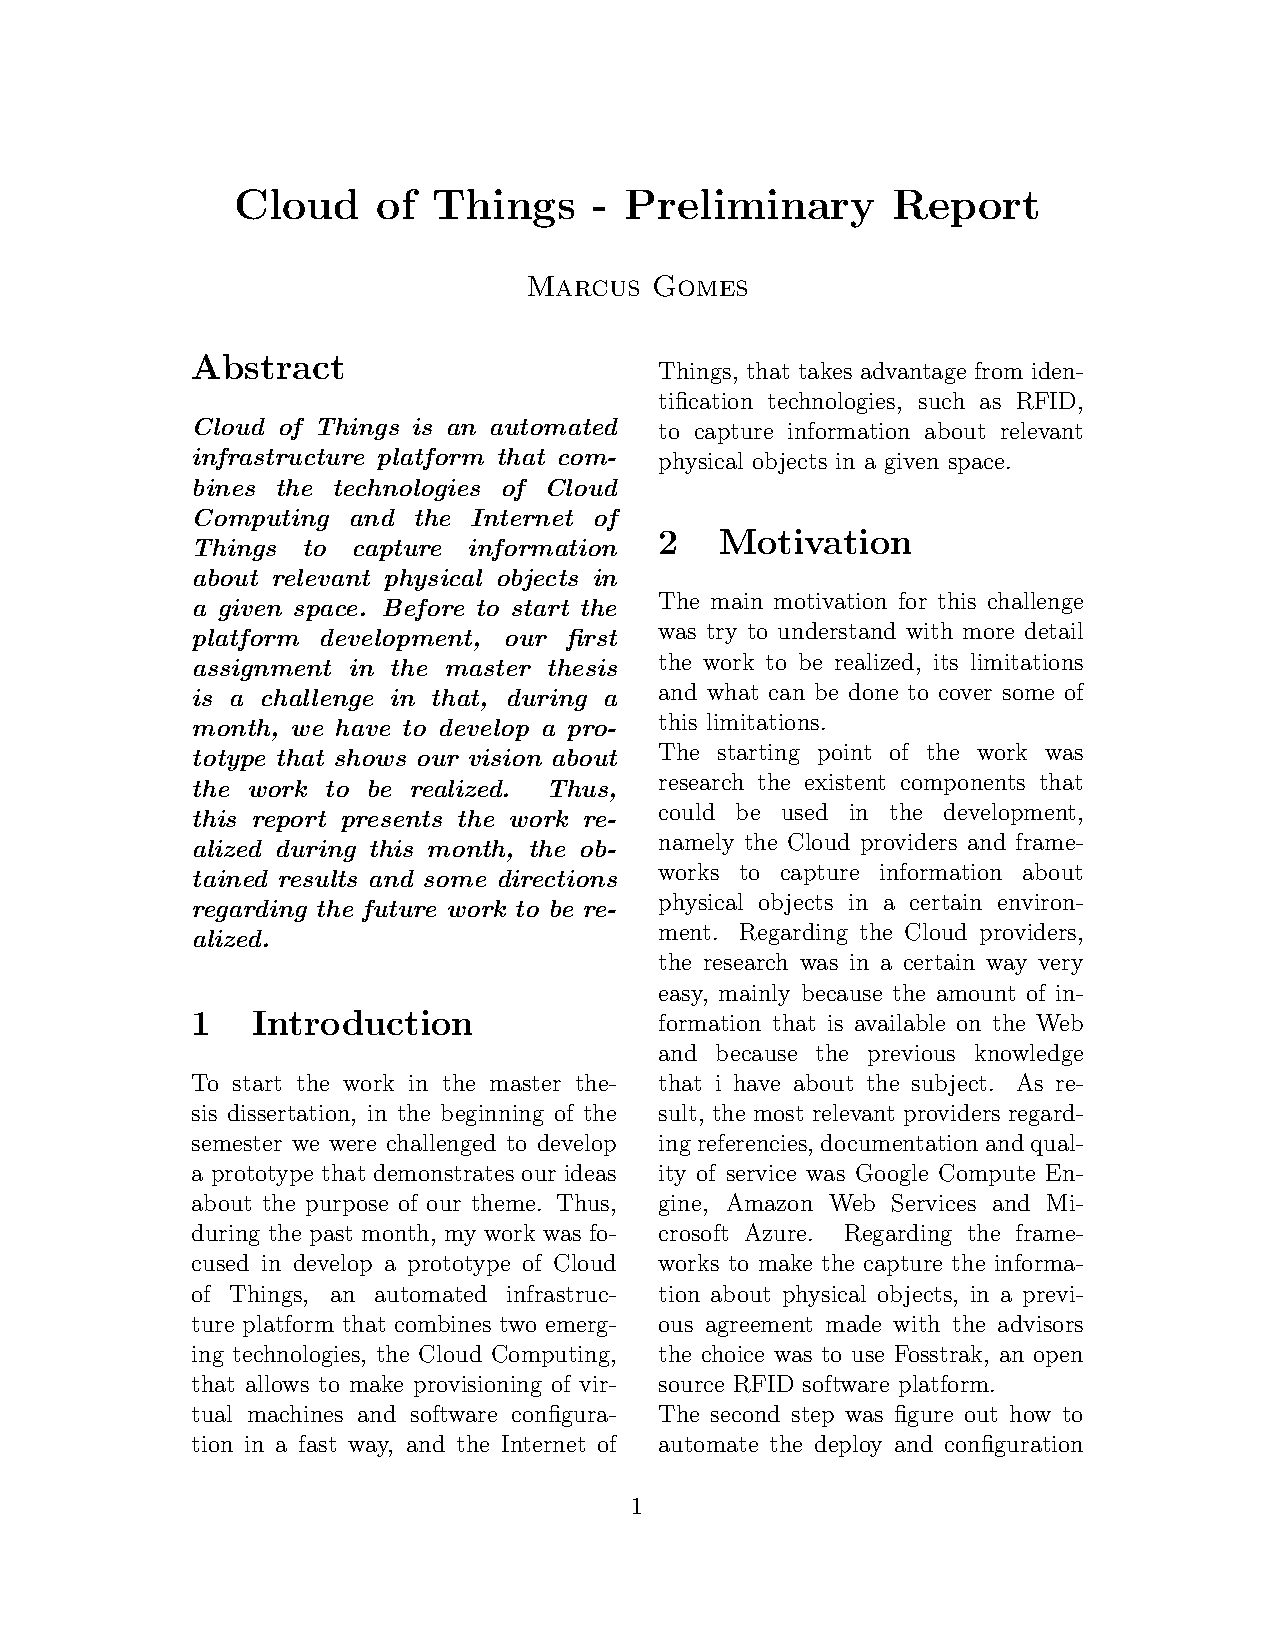
\includegraphics[width=.45\textwidth]{cot}
    \caption{Demo Scenario}
    \label{fig:demo}
 \end{figure}
 
 During the demonstration the Internet connection was too slow, and because that the demonstration fails. Although this situation reveals a possible problem to be explored, a low bandwidth network could preclude the procedure. Thus, it's important know how
 much data Puppet framework sends to the Cloud, because the problem could be there.\\
 After the demonstration the advisors make some important observations about was presented and about the future work that can be realized, as listed as follows:
 \begin{itemize}
 \item
 The Smart Space definition is too vague, the context of what is a Smart Space must be defined.
 \item
 The system user must be defined, the user is a \textit{Power User} or not. This is important to establish the abstraction level of the application.
 \item
 Regarding the \textbf{Cloud Server} deployment, there are models to determine the amount of resources that is needed for a given space?
 \item
 Regarding the \textbf{Status Check}, what is the Service Level Agreements (SLA's) established by the Cloud providers?     
 \end{itemize}   
 % -----------------------------------------------------------------------------------------------
 % CONCLUSION
 % -----------------------------------------------------------------------------------------------
 \section{Conclusion}
 This experimentation process was very important, because allowed us to understand the context of our work and what is the future work that can be realized. Personally, was very satisfying because now i'm sure that i choose the right theme.\\
 For the future, the first thing to do is pick on the observations pointed at the prototype demonstration and start to structure the \textit{Dissertation Question} in a more concise way, beginning with the definition of: \textbf{What is a Smart Space}? 
\end{document}  